%!TEX TS-program = Arara
% arara: lualatex
% https://tex.stackexchange.com/questions/425098/which-opentype-math-fonts-are-available
\documentclass[11pt,parskip=half,DIV=12,ngerman]{scrartcl}

\usepackage{babel}
\usepackage{amsmath}
\usepackage{amsthm}
\usepackage{nicefrac,array}
\usepackage{blindtext}
\usepackage{tikz}
\usetikzlibrary{arrows}
\usetikzlibrary{lindenmayersystems}
\usepackage{microtype}

\usepackage{amsmath}
\DeclareMathOperator\Res{Res}
\newcommand*\diff{\mathop{}\!\mathup{d}}

\usepackage{unicode-math}

\setmainfont{EBGaramond-Regular}[
  BoldFont = EBGaramond-Bold,
  ItalicFont = EBGaramond-Italic,
  BoldItalicFont = EBGaramond-BoldItalic
]
\setmathfont{Garamond Math}[Scale=MatchUppercase]

\begin{document}

\blindtext[1]

{\setlength{\extrarowheight}{0.5em}
\begin{equation}
\left\{
\begin{array}{l}
p = - \frac{5}{3} P^3 \left\{A \frac{\delta^2 \left(\frac{1}{\rho} \right)}{\delta \xi^2} + B  \frac{\delta^2 \left(\frac{1}{\rho} \right)}{\delta \eta\,^2} + C \frac{\delta^2 \left(\frac{1}{\rho} \right)}{\delta \zeta\,^2} \right\} + \text{konst.}, \\
u = A \xi - \frac{5}{3} P^2 A \frac{\xi}{\rho^3} - \frac{\delta D}{\delta \xi}, \\
v = B \eta - \frac{5}{3} P^3 B \frac{\eta}{\rho^3} - \frac{\delta D}{\delta \eta}, \\
w = C \zeta - \frac{5}{3} P^3 C \frac{\zeta}{\rho^3} - \frac{\delta D}{\delta \zeta},
\end{array}
\right.\label{eq5}
\end{equation}
}

\pgfdeclarelindenmayersystem{Hilbert curve}{
  \rule{L -> +RF-LFL-FR+}
  \rule{R -> -LF+RFR+FL-}}

\begin{center}
  \begin{tikzpicture}[scale=30]
      \begin{scope}[xshift=.5*7 cm,yshift=0cm,rotate=0, scale = 1/(2^(7)-1)]
        \shadedraw [bottom color=white, top color=white, draw=red]
        [l-system={Hilbert curve, axiom=L, order=5, step=8pt, angle=90}]
        lindenmayer system;
      \end{scope}
  \end{tikzpicture}
\captionof{figure}{Aus dem \texttt{lindenmayersystems} Paket}
\end{center}

\begin{center}
\fbox{%
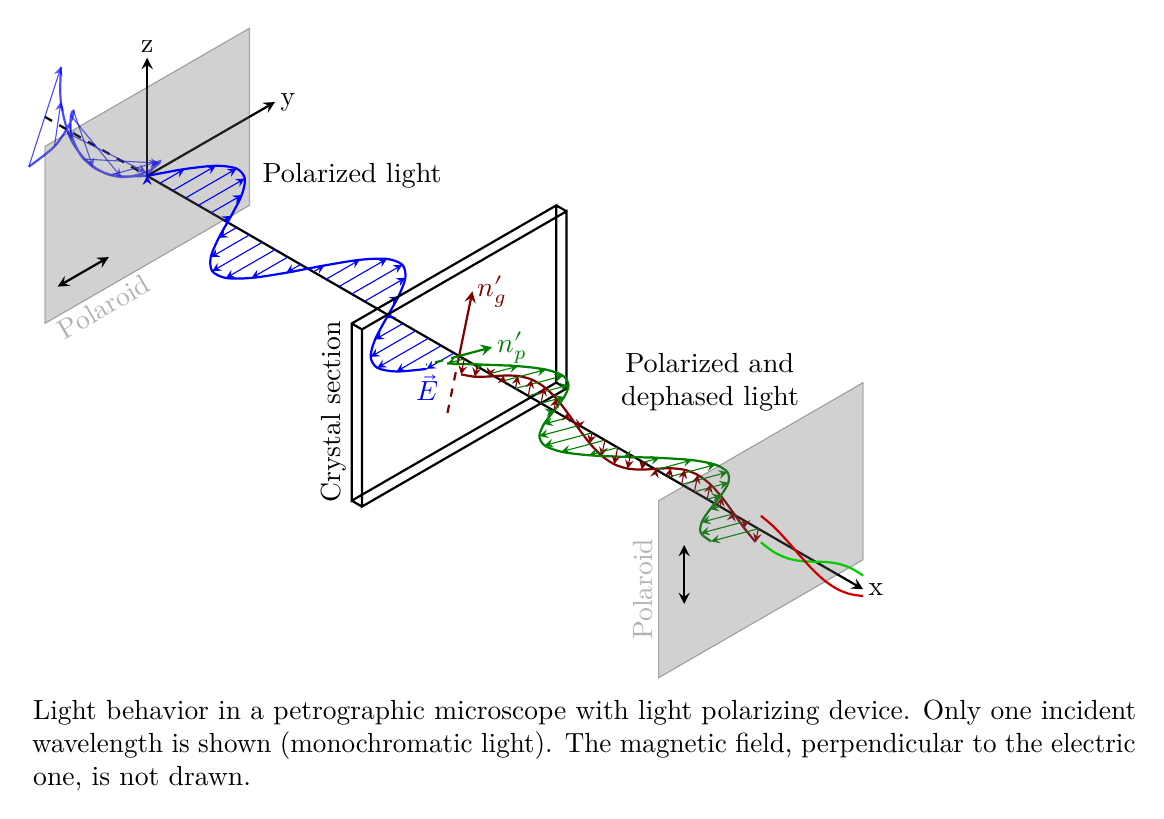
\begin{tikzpicture}[x={(0.866cm,-0.5cm)}, y={(0.866cm,0.5cm)}, z={(0cm,1cm)}, scale=0.75,
    %Option for nice arrows
    >=stealth, %
    inner sep=0pt, outer sep=2pt,%
    axis/.style={thick,->},
    wave/.style={thick,color=#1,smooth},
    polaroid/.style={fill=black!60!white, opacity=0.3},
]
    % Colors
    \colorlet{darkgreen}{green!50!black}
    \colorlet{lightgreen}{green!80!black}
    \colorlet{darkred}{red!50!black}
    \colorlet{lightred}{red!80!black}

    % Frame
    \coordinate (O) at (0, 0, 0);
    \draw[axis] (O) -- +(14, 0,   0) node [right] {x};
    \draw[axis] (O) -- +(0,  2.5, 0) node [right] {y};
    \draw[axis] (O) -- +(0,  0,   2) node [above] {z};

    \draw[thick,dashed] (-2,0,0) -- (O);

    % monochromatic incident light with electric field
    \draw[wave=blue, opacity=0.7, variable=\x, samples at={-2,-1.75,...,0}]
        plot (\x, { cos(1.0*\x r)*sin(2.0*\x r)}, { sin(1.0*\x r)*sin(2.0*\x r)})
        plot (\x, {-cos(1.0*\x r)*sin(2.0*\x r)}, {-sin(1.0*\x r)*sin(2.0*\x r)});

    \foreach \x in{-2,-1.75,...,0}{
        \draw[color=blue, opacity=0.7,->]
            (\x,0,0) -- (\x, { cos(1.0*\x r)*sin(2.0*\x r)}, { sin(1.0*\x r)*sin(2.0*\x r)})
            (\x,0,0) -- (\x, {-cos(1.0*\x r)*sin(2.0*\x r)}, {-sin(1.0*\x r)*sin(2.0*\x r)});
    }

    \filldraw[polaroid] (0,-2,-1.5) -- (0,-2,1.5) -- (0,2,1.5) -- (0,2,-1.5) -- (0,-2,-1.5)
        node[below, sloped, near end]{Polaroid};%

    %Direction of polarization
    \draw[thick,<->] (0,-1.75,-1) -- (0,-0.75,-1);

    % Electric field vectors
    \draw[wave=blue, variable=\x,samples at={0,0.25,...,6}]
        plot (\x,{sin(2*\x r)},0)node[anchor=north]{$\vec{E}$};

    %Polarized light between polaroid and thin section
    \foreach \x in{0, 0.25,...,6}
        \draw[color=blue,->] (\x,0,0) -- (\x,{sin(2*\x r)},0);

    \draw (3,1,1) node [text width=2.5cm, text centered]{Polarized light};

    %Crystal thin section
    \begin{scope}[thick]
        \draw (6,-2,-1.5) -- (6,-2,1.5) node [above, sloped, midway]{Crystal section}
                -- (6, 2, 1.5) -- (6, 2, -1.5) -- cycle % First face
            (6,  -2, -1.5) -- (6.2, -2,-1.5)
            (6,   2, -1.5) -- (6.2,  2,-1.5)
            (6,  -2,  1.5) -- (6.2, -2, 1.5)
            (6,   2,  1.5) -- (6.2,  2, 1.5)
            (6.2,-2, -1.5) -- (6.2, -2, 1.5) -- (6.2, 2, 1.5) 
                -- (6.2, 2, -1.5) -- cycle; % Second face

        %Optical indices
        \draw[darkred, ->]       (6.1, 0, 0) -- (6.1, 0.26,  0.966) node [right] {$n_{g}'$}; % index 1
        \draw[darkred, dashed]   (6.1, 0, 0) -- (6.1,-0.26, -0.966); % index 1
        \draw[darkgreen, ->]     (6.1, 0, 0) -- (6.1, 0.644,-0.173) node [right] {$n_{p}'$}; % index 2
        \draw[darkgreen, dashed] (6.1, 0, 0) -- (6.1,-0.644, 0.173); % index 2
    \end{scope}

    %Rays leaving thin section
    \draw[wave=darkred,   variable=\x, samples at={6.2,6.45,...,12}] 
        plot (\x, {0.26*0.26*sin(2*(\x-0.5) r)},  {0.966*0.26*sin(2*(\x-0.5) r)});  %n'g-oriented ray
    \draw[wave=darkgreen, variable=\x, samples at={6.2,6.45,...,12}]
        plot (\x, {0.966*0.966*sin(2*(\x-0.1) r)},{-0.26*0.966*sin(2*(\x-0.1) r)}); %n'p-oriented ray
    \draw (10,1,1) node [text width=2.5cm, text centered] {Polarized and dephased light};

    \foreach \x in{6.2,6.45,...,12} {
        \draw[color=darkgreen, ->] (\x, 0, 0) --
            (\x, {0.966*0.966*sin(2*(\x-0.1) r)}, {-0.26*0.966*sin(2*(\x-0.1) r)});
        \draw[color=darkred,   ->] (\x, 0, 0) --
            (\x, {0.26*0.26*sin(2*(\x-0.5) r)}, {0.966*0.26*sin(2*(\x-0.5) r)});
    }

    %Second polarization
    \draw[polaroid]   (12, -2,  -1.5) -- (12, -2,   1.5)  %Polarizing filter
        node [above, sloped,midway] {Polaroid} -- (12, 2, 1.5) -- (12, 2, -1.5) -- cycle;
    \draw[thick, <->] (12, -1.5,-0.5) -- (12, -1.5, 0.5); %Polarization direction

    %Light leaving the second polaroid
    \draw[wave=lightgreen,variable=\x, samples at={12, 12.25,..., 14}]
        plot (\x,{0}, {0.966*0.966*0.26*sin(2*(\x-0.5) r)}); %n'g polarized ray
    \draw[wave=lightred,  variable=\x, samples at={12, 12.25,..., 14}]
        plot (\x,{0}, {-0.26*0.966*sin(2*(\x-0.1) r)});      %n'p polarized ray

    \node[align=justify, text width=14cm, anchor=north west, yshift=-2mm] at (current bounding box.south west)
        {Light behavior in a petrographic microscope with light polarizing
        device. Only one incident wavelength is shown (monochromatic light).
        The magnetic field, perpendicular to the electric one, is not drawn.};
\end{tikzpicture}}
\captionof{figure}{Quelle: https://texample.net/tikz/examples/polarizing-microscope/}
\end{center}


\end{document}
